\documentclass[a4paper, UKenglish, 11pt]{uiomaster}
\usepackage{lipsum}
\usepackage[subpreambles=true]{standalone}


\begin{document}
\chapter{Methods}
\section{New York Head Model}
The New York Head Model is a computer model of the human head used to simulate the electrical activity of the brain. It was created by the Electrical Geodesics Incorporated (EGI) in 2004, and is based on the anatomical and electrical characteristics of the head of a typical adult human.

The model consists of a three-dimensional (3D) representation of the head and brain, with detailed information on the geometry and electrical properties of the different tissues and structures within the head. The model includes the scalp, skull, cerebrospinal fluid, gray matter, and white matter. The electrical properties of each of these tissues, such as conductivity and permittivity, are also included in the model.

The New York Head Model is used in research and clinical applications to understand the electrical activity of the brain and diagnose neurological disorders. It is particularly useful for studying the electrical activity of the brain during various cognitive and motor tasks, as well as during seizures and other abnormal brain activity.

The model is also used in the field of non-invasive brain stimulation, where it helps to guide the placement of electrodes or magnetic coils to target specific areas of the brain for therapeutic or diagnostic purposes. By using the model to predict the electrical activity of the brain, researchers and clinicians can optimize the placement of the electrodes or magnetic coils to achieve the desired effect.

Overall, the New York Head Model is an important tool for understanding the electrical activity of the brain and has numerous applications in research and clinical settings.

\section{Machine Learning and Neural Networks}
Computational neuroscience is a field that aims to understand the principles underlying information processing in the brain using mathematical and computational tools. The inverse problem in EEG, which involves estimating the location and strength of electrical sources in the brain based on measurements of electrical activity on the scalp, is a key challenge in computational neuroscience. Machine learning techniques, including feedforward neural networks, have been used to address this problem by learning to map the measured EEG signals to estimates of the underlying electrical sources in the brain.

Source localization using machine learning techniques has shown promise for improving the accuracy and efficiency of EEG analysis, and has been applied to a variety of cognitive and clinical applications. For example, machine learning-based source localization has been used to study the neural mechanisms underlying attention, memory, and perception (Wu et al., 2018; Lopes da Silva et al., 2019), as well as to diagnose and monitor neurological disorders such as epilepsy (Safieddine et al., 2019; Shah et al., 2020). These applications demonstrate the potential of machine learning and computational neuroscience to enhance our understanding of the brain and improve clinical outcomes.

Machine learning is a field of computer science that involves using algorithms and statistical models to enable computers to learn from data without being explicitly programmed. One popular type of machine learning algorithm is the feedforward neural network, which is a type of artificial neural network that is often used for tasks such as linear regression. In a feedforward neural network, data is passed through a series of layers of interconnected nodes, or "neurons," which perform mathematical operations to transform the data.

Linear regression is a common machine learning task that involves predicting a continuous quantity, such as the price of a house or the temperature of a city, based on a set of input features. In a feedforward neural network, linear regression can be accomplished by using a single neuron in the output layer of the network that computes a weighted sum of the input features and applies an activation function to produce the predicted output value. The weights on the input features are learned by the network during the training process, which involves adjusting the weights to minimize the difference between the predicted output values and the actual output values in the training data.

Overall, feedforward neural networks are a powerful machine learning tool that can be used to solve a wide range of problems, including linear regression. By adjusting the weights and biases of the neurons in the network during the training process, neural networks can learn to make accurate predictions based on input data, making them a valuable tool for a variety of applications.

% References:
%
% Lopes da Silva, F. H., Da Silva, F. L., Blanes, W., & Kalitzin, S. N. (2019). Towards a functional definition of epileptic networks. Epilepsy & behavior, 102, 106643.
%
% Safieddine, D., Murai, K. K., Tsakalis, K. S., & Valiante, T. A. (2019). Dynamic source localization of epileptic spikes using a recurrent neural network. Frontiers in neuroscience, 13, 1352.
%
% Shah, P., Taylor, P. N., & Worrell, G. A. (2020). Automatic detection and localization of seizures in intracranial electroencephalographic recordings using deep learning. Journal of neural engineering, 17(1), 016015.
%
% Wu, T., Li, H., He, B., & Li, Y. (2018). A review of techniques for detecting and localizing EEG abnormalities. Journal of neuroscience methods, 302, 44-57.




​





% \section*{Machine Leaning}
% The fit is found using the method of least squares using polynomials x and y up to the eighth order. The mean square error (MSE) can be used to evaluate how well the model fit our data, which is given by:
%
% \begin{equation}
% MSE(\hat{y},\hat{\tilde{y}}) = \frac{1}{n}
% \sum_{i=0}^{n-1}(y_i-\tilde{y}_i)^2
% \label{eq:MSE}
% \end{equation}
%
% Where $\tilde{y}_i$ is the predicted value and $y_i$ is the corresponding true value. Having a MSE of zero, would mean that the estimator $\hat{y}$ predicts observations of the parameter $\hat{\tilde{y}}$ with perfect accuracy. This is obviously ideal, but is however, not typically possible.
%
% The predicted value $\tilde{y}_i$ can be rewritten as $\tilde{y}_i=x_i^T\beta$, which we can use to find the residual sum of the squares:
%
% \begin{equation}
% RSS(\beta) =
% \sum_{i=1}^{N}(y_i-x_i^T\beta)^2
% \label{eq:RSS}
% \end{equation}
%
% The ordinary least squares method (OLS) wants to minimize the sum of the residuals, which is given by the RSS value (see equation \ref{eq:RSS}). We want to find the $\beta$ which minimize this function. If we define a $N \times p$ matrix $\textbf{X}$ with each row as an input vector and a N-vector $\textbf{y}$ of the true values, we can represent our solution $\hat{\beta}$ as a 1-dimensional array of size p using matrix notation:
%
% \begin{equation}
% \hat{\beta}=(\textbf{X}^T\textbf{X})^{-1}\textbf{X}^T\textbf{y}
% \label{eq:beta}
% \end{equation}
%
% where $\textbf{X}^T\textbf{X}$ is non singular \cite{94}. The size of $\hat{\beta}$ will depend on the degree of our polynomial fit. For example polynomial degree 5 we will give us a $\hat{\beta}$ length of p=21. The length N is given by the number of datapoints. % remember to plug in the equation for finding the length of the beta-vector
%
% Just like MSE, the coefficient of determination $R^2$ is a measure for how precise a model is. To be more precise, it provides a measure of how well future samples are likely to be predicted by the model. The score normally ranges between 0 and 1, where 1 is the best possible score. In general, the higher the R-squared, the better the model fits the data. The coefficient of determination $R^2$ is given as follows:
% %skrive litt mer om r2-score?
% \begin{equation}
% R^2(\hat{y}, \tilde{\hat{y}}) = 1 - \frac{\sum_{i=0}^{n - 1} (y_i - \tilde{y}_i)^2}{\sum_{i=0}^{n - 1} (y_i - \bar{y})^2},
% \label{eq:R2}
% \end{equation}
%
% Where the mean value of $y_i$ is defined by $\bar{y}$:
%
% \begin{equation*}
% \bar{y} =  \frac{1}{n} \sum_{i=0}^{n - 1} y_i.
% \label{eq:ybar}
% \end{equation*}
%
% Creating a perfect model for a set of data, can easily be done by using a high polynomial degree when fitting. However, creating a foolproof model that only fits one specific data set is not very beneficial. We want our model to predict correlated data, not slavishly follow the path of least square error. With this in mind we should split our data into training and testing sets in order to make the model compatible with multiple data sets. By splitting our data we can test how well our model predicts. In this exercise we have chosen to train on $80\%$ of our data, and test on the remaining $20\%$. By training, in this context, we mean to find the $\beta$ that minimize the cost function, using the training data. Having obtained $\hat{\beta}$ we test our model on both sets, expecting that it fits well for both the training and test data.
%
% A much used approach before starting to train the data is to scale our data. The data may be very sensitive to extreme values, and scaling the data could render our inputs more suitable for the algorithms we want to use.
%
% There are several methods for scaling data sets. In this project we have scaled our data by calculating the mean and standard deviation for each feature. For each observed value of the feature, we subtract the mean and divide by the standard deviation. The first feature (first column in our design matrix) was kept untouched, in order to avoid singularities when calculating $\beta$. This sort of scaling is called “Standardizing”. When standardizing data one obtain a "standard normal" random variable with mean 0 and standard deviation 1 \cite{96}.
%
% If any, there are very few data sets in the real world which have ideal properties without noise. When generating our own data set for the Franke function we therefore explore the addition of an added normal distributed $N(0,1)$ stochastic noise, in order to make the data set more realistic.
%
% \subsection*{Gradient Descent}
%
% When training an algorithm one wants to minimize the cost function to reach its global minimum. Instead of using matrix inversion to reach this minimum we now want to use gradient descent. This is useful due to the fact that it sometimes is hard to perform matrix inversion on data sets.
%
% Gradient Descent is an optimization algorithm for finding a local minimum of a derivable function. The underlying idea of the algorithm is that a function $F(\textbf{x})$ decreases fastest if we take repeated steps in the opposite direction of the negative gradient $-\nabla F(\textbf{x})$ of the function at $\textbf{x}$. We have that:
%
% \begin{equation}
%     \textbf{w}_{k+1} = \textbf{w}_k - \eta_k\nabla F(\textbf{w}_k)
%     \label{eq:GD}
% \end{equation}
%
% which leads to $F(\textbf{w}_{k+1}) \leq F(\textbf{w}_{k})$, when $\eta_k > 0$. This means that for sufficiently small step lengths $\eta_0$ we are always moving towards a minimum. In the Gradient Descent method we do an initial guess on weights $\textbf{w}_0$ and compute new approximations according to equation \ref{eq:GD}.
%
% Gradient descent then starts at a point and takes steps in the steepest downside direction until it reaches the point where the cost function is as small as possible.
%
% It is important to note that GD is very sensitive to the chosen initial condition. In machine learning we often deal with non-convex high dimensional cost functions with many local minima. This means, that unless we have a very good initial guess, we risk getting stuck in a local minimum when the gradient converges. Moreover, the algorithm is sensitive to the step length $\eta_0$, also referred to as the learning rate. If we take too large steps, we risk stepping over the global minimum point, resulting in unpredictable behavior. The step length also needs to be large enough so we don't get "stuck" in a local minimum point. Another fact is that a small learning rate will require many iterations before we reach a minimum point, which increases CPU time.
%
% One common problem with the GD method is that it has a tendency to overshoot the exact minimum. It has been shown that by slowly decreasing the learning rate we will obtain convergence behaviour similar to the batch gradient descent, which can help it converge towards a local or global minimum point \cite{100}. We define a learning rate function which adjust as a function of a variable t, which is proportional to the number of epochs. The learning rate function is given by:
%
% \begin{equation}
%     \eta(t)=\frac{t_0}{t+t_1}
% \label{eq:learning_rate_func}
% \end{equation}
%
% Where $t_0$ and $t_1$ are constants. This equation will decrease as we run through our batches, since we are dividing by the t term. In Scikit-Learn's "SGDRegressor" we have that $t_1=\frac{1}{0.01*t_0}$, which we use in our own model when we compare with the method provided in Scikit-Learn.
%
% %Furthermore, we mark that gradient as a function of $\textbf{x} = (x_1, x_2, ..., x_n)$ which makes it expensive to compute numerically. The method named Stochastic Gradient descent alleviates some of these problems by introducing randomness.
%
% \subsubsection*{Stochastic Gradient Descent with momentum}
%
% In almost all cases we can write our cost function as a sum over $n$ data points:
%
% \begin{equation}
%     C(\beta) = \Sigma^{n}_{i=1}c_i(\textbf{x}_i, \beta).
% \end{equation}
%
% Which means that the total gradient can be computed as a sum over i -gradients:
%
% \begin{equation}
%     \nabla_\beta C(\beta) = \Sigma^n_i\nabla_\beta c_i(\textbf{x}_i, \beta)
%     \label{eq:SGD}
% \end{equation}
%
% % Checkpoint
%
% The SGD method allows us to take the gradient on randomly selected subsets of data at every step rather than the full data set. These subsets are commonly referred to as mini-batches. In other words, Stochastic Gradient Descent is just like regular Gradient Descent, except it only looks at one mini-batch for each step. The mini-batches are denoted by $B_k$ where k runs from 1 and up to the number of batches, $n/M$. An iteration over the number of mini-batches is called an epoch.
%
% Introducing randomness by only taking the gradient on a subset of the data, is beneficial as it lowers the chance of getting stuck in a local minimum point. Moreover, splitting the data points into batches reduces the time spent calculating the derivatives of the cost function, since we sum over $k$ batches and not all $n$ data points.
% Implementing momentum to the Stochastic Gradient Descent, helps accelerate gradient vectors in the right directions, which leads to faster converging. In many ways this improves the algorithms sensitivity to the learning rate. The momentum serves as a memory of the direction we are moving in parameter space and can be written as follows:
%
% \begin{equation}
%     \textbf{v}_{t} = \gamma\textbf{v}_{t-1} - \eta_t\nabla F(\boldsymbol{\beta}_t)
%     \label{eq:GDM}
% \end{equation}
%
% \begin{equation}
%     \boldsymbol{\beta}_{t+1} = \boldsymbol{\beta}_t - \textbf{v}_t
%     \label{eq:GDM_beta}
% \end{equation}
%
% where the parameter $\gamma$ represents the momentum and must be between 0 and 1. The momentum term $\gamma$ is usually set to 0.9 or a similar value \cite{100}. We used $\gamma = 0.9$. We also set the initial "velocity" to $v=0$.
%
% \subsubsection*{The momentum SGD algorithm}
% \begin{algorithmic}[H]
% \label{sudo:MSGD}
% \\
% \State \textit{Initialize all the parameters.}
% \State \textit{Create design matrix $X$}
% \State \textit{Call Franke's Function with $x$ and $y$. This is our $z$.}
% \State \textit{Guess on some $\beta$ values.}
% \For { $epoch \in \{N_{epochs}\}$}
% \State \textit{Shuffle the data}
% \For { $index \in \{m_{minibatches}\}$}
% \State \textit{Calculate gradients}
% \State \textit{Find current learning rate}
% \State \textit{$v = \gamma * v + \eta *$ gradients}
% \State \textit{$\beta = \beta - v$}
%
% \end{algorithmic}
% \\
% For the ordinary SGD method we have one less term in the loop over minibatches: \textit{$\beta = \beta - \eta * gradients$}.
%
%
% \subsection*{Neural  Networks}
% %Gradient descent is the preferred way to optimize neural networks.
% Artificial Neural Networks are computational systems that can learn to perform tasks by considering examples, generally without being programmed with any task-specific rules \cite{101}.
%
% The biological neural networks of animal brains, wherein neurons interact by sending signals in the form of mathematical functions between layers, has inspired a simple model for an artificial neuron:
%
% \begin{equation*}
%     a = f \left( \Sigma_{i=1}^n w_ix_i + b_i\right ) = f(z)
%     \label{eq:NN}
% \end{equation*}
%
% where the output $a$ of the neuron is the value of its activation function $f$, which as input has the sum of signals $x_i, x_{i+1}, ..., x_n$ received by $n$ other neurons, multiplied with the weights $w_i, w_{i+1}, ..., w_n$ and added with biases.
%
% Most artificial neural networks consists of an input layer, an output layer and layers in between, called hidden layers. The layers consists of an arbitrary number of neurons, also referred to as nodes. The connection between two nodes is associated with a weight variable $w$, that weights the importance of various inputs. A more convenient notation for the activation function is:
%
% \begin{equation}
%     a_i(\boldsymbol{x}) = f_i(z^{(i)}) = f_i(\boldsymbol{w^{i}}\cdot \boldsymbol{x} + b^{i})
% \label{eq:NN_vec}
% \end{equation}
%
% where $\boldsymbol{w}^{(i)} = (w_1^{(i)}, w_2^{(i)}, ..., w_n^{(i)})$ and $b^{(i)}$ are the neuron-specific weights and biases respectively. The bias is normally needed in case of zero activation weights or inputs \cite{101}.
%
% \subsubsection*{Feed Forward Neural Network}
%
% As the name name suggests, in Feed Forward Neural Network (FFNN) the information only moves in one direction, forward through layers. This means that in an FFNN, the inputs $x_i$ of the activation function $f$ are the outputs of the neurons in the preceding layer.
%
% The Universal Approximation Theorem tells us that no matter what our data set is, there is a Neural Network that can approximately approach the result and do the job. This result holds for any number of inputs and outputs \cite{95}.
%
% Thus the basic components of a neural network are stylized neurons consisting of a linear transformation that weights the importance of various inputs, followed by a non-linear activation function. A typical example for such an activation function is the logistic Sigmoid (\ref{eq:Sigmoid}).
%
% We assume that there are $L$ layers in our network with $l = 1,...,L$ indexing the layer and that different layers have different activation functions. Further we denote $w^l_{ij}$ as the weight for the connection from the $j$-th neuron in layer $l-1$ to the $i-th$ neuron in layer $l$. The bias of this neuron is written as $b^l_i$. The mathematical model for a FFNN is then reads:
% \begin{equation}
%     a_i^l = f^l(z_i^l) = f^l \left(\Sigma_{j=1}^{N_{l-1}}w_{ij}^l a_j^{l-1} + b_i^l\right)
% \label{eq:FFNN}
% \end{equation}
% where $l$ denotes the $l$-th layer and $N_l$ is the number of nodes in layer $l$. A FFNN that is fully-connected consisting of neurons that have non-linear activation functions, receives a weighted sum of the outputs of all neurons in the previous layer (figure \ref{fig:FFNN}). %--> Regnte med at det var denne du mente
%
% %\begin{figure}[H]
% %    \centering
% %    \includegraphics[width=\linewidth]{FFNN.png}
% %    \caption{In \textbf{A} we see that one data point from the input data  is connected (as visualized in \textbf{A}) to all neurons in the following layer. This process goes on until we reach the output layer.}
% %    \label{fig:FFNN}
% %\end{figure}
%
% We will be studying Franke's function which produces a certain type of terrain data. You can read more about Franke's function in our previous report \cite{97}.
%
% % Here: linear means that each node in the output layer has a linear activation function.
% % find picture to illustrate
%
% \subsubsection*{Back propagation algorithm}
%
% The back propagation algorithm is a clever procedure that allows us to change the weights in order to minimize the cost function. At its core, back propagation is simply the ordinary chain rule for partial differentiation, and can be summarized using four equations \cite{96}.
%
% The fist equation is the definition of the error $\delta_i^L$ of the $i$-th neuron in the $L$-th layer:
%
% \begin{equation}
%     \delta_i^L = \frac{\partial C}{\partial(z_i^L)},
% \label{eq:I}
% \end{equation}
% which can be thought of as the change to the cost function by increasing $z_i^L$ infinitesimally. By definition, the cost function measures the error of the output compared to the target data. So if the error $\delta_i^L$ is large, that would suggest the cost function hasn't yet reached its minima.
% The second equation is the analogously defined error of neuron $i$ in layer $l$, $\delta_i^l$:
% \begin{equation}
%     \delta_i^l = f'(z_i^l)\frac{\partial C}{\partial(a_i^l)}
% \label{eq:II}
% \end{equation}
% where $f'(z_i^l)$ measures how fast the activation function $f$ is changing at the given activation value.
% Utilizing that $\delta_i^l = \frac{\partial C}{\partial z_j^l}$ we can express the error in terms of the equations for layer $l+1$. This can be done by using the chain rule, and is the third back propagation equation (for full calculations see \cite{102} under "Final back propagation equation"):
%
% \begin{equation}
%     \delta_i^l = \frac{\partial C}{\partial z^l_{i}} = \Sigma \delta_j^{l+1}w_{ij}^{l+1}f'(z_i^l)
% \label{eq:III}
% \end{equation}
%
% Finally the last equation of the four back propagation equations the derivative of the cost function in terms of the weights:
%
% \begin{equation}
%     \frac{\partial C}{\partial w^l_{ij}} = \delta_i^l a_j^{l-1}
% \label{eq:IV}
% \end{equation}
%
% With these four equations in hand we can now calculate the gradient of the cost function, starting from the output layer, and calculating the error of each layer backwards. We then have a way of adjusting all the weights and biases to better fit the target data. The back propagation algorithm then goes as follows:
%
% \begin{enumerate}
%   \item \textbf{Activation at input layer:} calculate the activations $a_i^1$ of all the neurons in the input layer.
%   \item \textbf{Feed forward:} starting with the first layer, utilize the feed-forward algorithm through \ref{eq:FFNN} to compute $z^{l}$ and $a^{l}$ for each subsequent layer.
%   \item \textbf{Error at top layer:} calculate the error of the top layer using equation \ref{eq:I}. This requires to know the expression for the derivative of both the cost function $C(\boldsymbol{W}) = C(\boldsymbol{a}^L)$ and the activation function $f(z)$.
%   \item \textbf{"Backpropagate" the error:} use equation \ref{eq:III} to propagate the error backwards and calculate $\delta_j^l$ for all layers.
%   \item \textbf{Calculate gradient:} use equation \ref{eq:II} and \ref{eq:IV} to calculate $\frac{\partial C}{\partial z^l_{i}}$ and $\frac{\partial C}{\partial w^l_{ij}} = \delta_i^l a_j^{l-1}$. \newline
%   \item \textbf{Update weights and biases:} \\[2pt] $w^l_{jk}=w^l_{jk}-\eta\delta^l_ja^{l-1}_k$ \\[2pt] $b_j^l = b_j^l - \eta \delta_j^l$
% \end{enumerate}
%
% \subsubsection*{Structure of our neural network}
%
% The way we decided to structure our neural network is based on how to handle the design matrix containing the input data used for producing Franke's Function terrain data. We decided to take a slightly different approach to setting up the design matrix compared to in project 1 \cite{97}. Instead of assuming a polynomial of a given complexity as we did there, we now set up the design matrix as shown below in (\ref{eq:design}). This way the columns represent all the $x$ and $y$ values respectively, and each row represent each its own unique combination of the input points. The design matrix then contains all the inputs used for producing the terrain, so by the universal approximation theorem there should then exist a network which should produce Franke's Function terrain. The design matrix then takes the form:
%
% \begin{equation}
% X=
%     \begin{bmatrix}
%         x_1 & y_1\\
%         x_2 & y_1 \\
%         . & . \\
%         . & . \\
%         x_n & y_1 \\
%         x_1 & y_2 \\
%         x_2 & y_2 \\
%         . & . \\
%         . & . \\
%         x_n & y_2 \\
%         . & . \\
%         . & . \\
%         x_1 & y_n \\
%         x_2 & y_n \\
%         . & . \\
%         . & . \\
%         x_n & y_n \\
%     \end{bmatrix}
% \label{eq:design}
% \end{equation}
%
% Where $n$ is the number of points in one direction. We then define the number of input rows as $N=n\times n$. We can visualize the feed forward method like this:
%
% \begin{figure}[H]
%     \centering
%     \includegraphics[width=\linewidth]{Feed_forward.png}
%     \caption{The feed forward method.}
%     \label{fig:our_FFNN}
% \end{figure}
%
% Where $w_i$ is the input weights and $w_o$ is the output weights. The numbered sub-indexes up to $L$ denote the hidden layers. $N$ is the input data points and $n_h$ is the number of hidden neurons. The superscripts denote the dimensions of the matrices. Notice how we have changed the order of the input-weight matrix multiplication when calculating the $z$'s. The reason for changing the order has to with making the dimensions add up, because when following the standard feed-forward formulas the dimensions didn't add up.
%
% For our neural network we choose the quadratic cost function with a Ridge regularization parameter ($L_2$-norm), described as follows:
%
% \begin{equation}
%     \frac{1}{2}\sum_{i=1}^{n}(a_i - t_i)^2 + \lambda||w||_2^2.
% \end{equation}
%
% The reason for choosing the quadratic loss function, as well as the $L_2$-norm, is their versatility and simple derivatives. When we look at the terrain data from Franke's function it is somewhat unnecessary to us regression models and resampling methods with the Ridge regularisation parameter. The reason was discussed in our previous report \cite{97}, which was that the lack of heavy outliers.
%
% However, when we are analyzing the breast cancer data set, we might expect more heavy outliers, which could benefit from a regularization parameter.
%
% \subsection*{Activation functions}
%
% The use of activation functions is inspired by the action potential of a human brain neuron; depending on the incoming current, the neuron will either fire or not. Activation functions work in a similar way, the input to a single neuron is transformed by an activation function causing a non-linear relation between the input and output. It is in this way the network learns. There are many activation functions, but the ones we will experiment with and discuss in this project are mainly:
%
% \begin{itemize}
%     \item The Sigmoid function: $f(z)=\frac{1}{1+e^{-z}}$
%     \item Hyperbolic tangent: $f(z)=\frac{e^{z}-e^{-z}}{e^{z}+e^{-z}}$
%     \item ReLU: $f(z)=\text{max}\{0,x\}$.
% \end{itemize}
%
% \subsubsection*{Sigmoid function}
%
% A big reason for using the Sigmoid is that it's range is between $[0, 1]$. This is naturally good when predicting probabilities. Another advantage when using the Sigmoid is that it is differentiable everywhere, where its analytical expression re-uses the sigmoid: $f'(x)=f(x)(1-f(x))$. This allows for effective computing in cases such as the back propogation algorithm which uses the derivative.
%
% \begin{figure}[H]
%     \centering
%     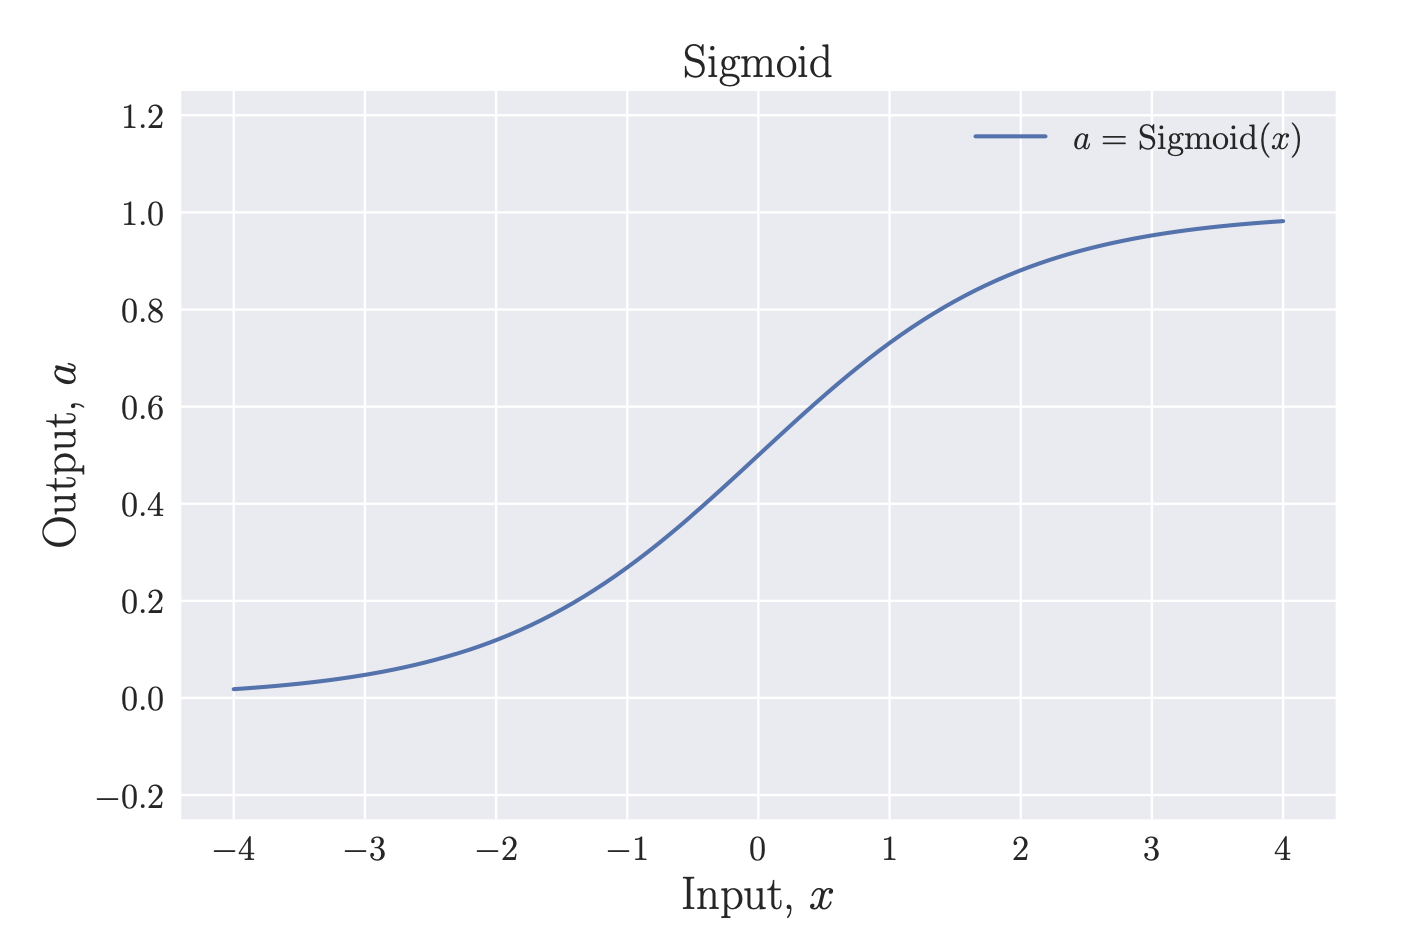
\includegraphics[width=80mm]{Task b,c/sigmoid.png}
%     \caption{We see the sigmoid with its characteristic S-shape and horisontal asymptotes at $1$ and $0$. Note that Sigmoid$(0)=0.5$.}
%     \label{fig:Sigmoid}
% \end{figure}
%
% \subsubsection*{Hyperbolic tangent (Tanh)}
% The hyperbolic tangent is similar to the Sigmoid in its shape and characteristics, but Tanh's range is instead between $[-1, 1]$ and Tanh$(0)=0$. Similar to the Sigmoid, Tanh also reuses itself in its expression for its derivative: $f'(x)=1-f(x)^2$
%
% \begin{figure}[H]
%     \centering
%     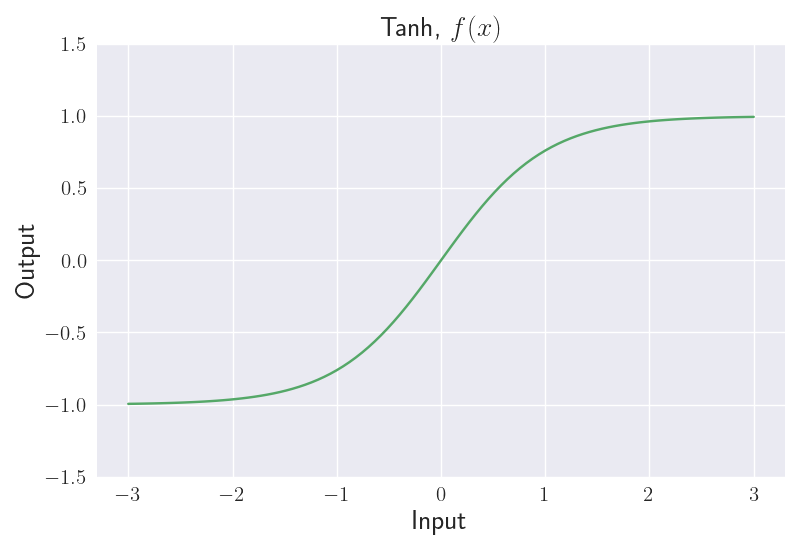
\includegraphics[width=80mm]{Task b,c/Tanh.png}
%     \caption{We see the hyperbolic tangent also with its characteristic S-shape, but with its horisontal asymptotes at $-1$ and $1$.}
%     \label{fig:Tanh}
% \end{figure}
%
% \subsubsection*{ReLU}
% ReLU is quite simple compared to the two mentioned above, in that it returns its input value if the input is above zero, and returns zero if the input is below zero. Its simplicity is one of the main reason for its wide usage in neural networks. For input values larger than zero it's also effective in avoiding vanishing gradients which the two others mentioned above are susceptible to (This will be discussed further in the next section). Though it must be noted that also the ReLU could be sucseptible to vanishing gradients given that the derivative for negative input values are zero. One minor problem when using ReLU is that it's not differentiable at $x=0$. This isn't necessarily a big problem as you can just define the derivative there to be zero, which is correct when $x$ approaches zero from the left. But it is something to be wary of when using the ReLU.
%
% \begin{figure}[H]
%     \centering
%     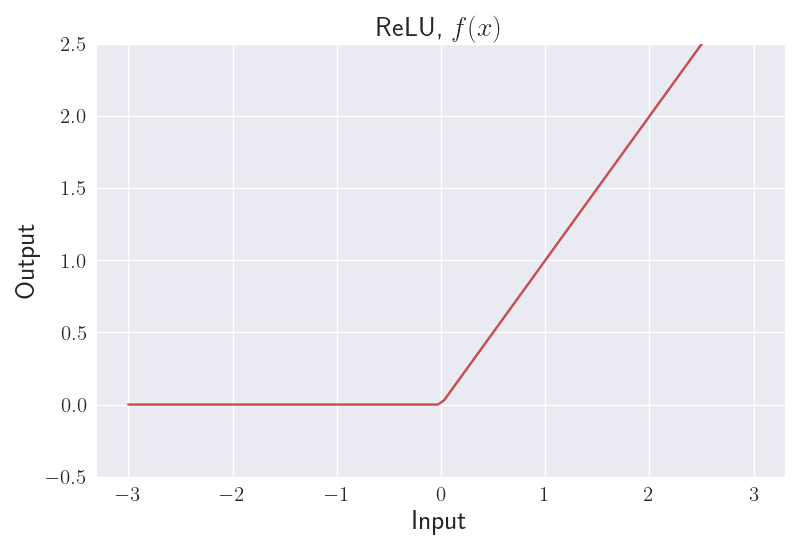
\includegraphics[width=80mm]{Task b,c/ReLU.png}
%     \caption{We see the ReLU with its non-differentiable sharp turn at $x=0$.}
%     \label{fig:ReLU}
% \end{figure}
%
% \subsection*{Initialization of the weights and biases}
%
% The initialization of the weights and biases is seemingly arbitrary, since the network in theory should change them accordingly to fit the target data. But there are naturally some initializations that will minimize the number of epochs necessary to reach convergence, and there are some that in practice won't reach convergence at all. The optimal choices of initialization will also depend on the chosen activation function in the network. Lets use the Sigmoid as an activation function as an example. If you choose very large, or very small weights, the gradient will become very small (figure \ref{fig:sigmoid}), causing the network to learn at an extremely slow rate. This is known as a vanishing gradient.
%
% However, by choosing a different activation function, say the ReLU or Tanh($x$), we might run into different problems. If we again initialize the weights to be very large, we can see that the derivative of the activation grows proportionally large (for certain areas) as the weights increase (figure \ref{fig:Exploding_gradients}), which in turn leads to what's normally called "exploding gradients". This problem will then only become worse as the number of layers are increased, though mainly for ReLU, since the proportionality factor from the weights carry through for each layer.
%
% The neural network can actually also experience exploding gradients when using the Sigmoid function. But if we were to use biases equal to zero as in the example above it wouldn't happen. This is because the Sigmoid is bounded between $0$ and $1$, with $\text{Sig}(0)=\frac{1}{2}$ and $\text{Sig}(1)\approx 0.73$. Thus, $\text{Sigmoid}(\text{Sigmoid}(x))$ is bounded between $0.5$ and $0.73$. As the number of layers increase, the resulting slope will then only become flatter and flatter. However, if a bias of value $b=\frac{w}{2}$ is added to the input in each layer, the gradient will start exploding, as shown in figure \ref{fig:exploding_sigmoid}. Though, it has to be noted that the chances of achieving such an exploding gradient when using the Sigmoid seems rather unlikely, as long as the weights and biases are not initialized in this specific way.
%
% \begin{figure}[H]
%     \centering
%     \includegraphics[width=\linewidth]
%     {Task b,c/sig_der_example.png}
%     \caption{The Sigmoid function and its derivative. We see that for large $x$-values the derivative converges towards zero.}
%     \label{fig:sigmoid}
% \end{figure}
%
% \begin{figure}[H]
%     \centering
%     \includegraphics[width=\linewidth]{Task b,c/ReLU_der_example.png}
%     \caption{In the figure above we can see that the derivatives grow proportionally large as the weights increase. The difference between the two functions can be seen as the derivative of Tanh only has one spike around $x=0$, while the derivative of the ReLU function is unbounded as $x\xrightarrow{}\infty$}.
%     \label{fig:Exploding_gradients}
% \end{figure}
%
% \begin{figure}[H]
%     \centering
%     \includegraphics[width=\linewidth]{Task b,c/sig_sig_der_example.png}
%     \caption{In the figure above we can see that when the input of the second layer is specified as $z=\text{Sig}(w\cdot x - w/2)$ the derivative starts to grow. This would continue to happen for each layer ultimately causing an exploding gradient. This is in contrast to using $b=0$ which would cause a vanishing gradient.}
%     \label{fig:exploding_sigmoid}
% \end{figure}
%
% \subsubsection*{The Xavier and Kaiper/He initialization methods.}
%
% From what we have discussed above, it seems that choosing reasonable initial weights and biases in combination with the right activation function is nothing other than a minefield impossible to navigate through. Luckily for us, there are people before us which have found methods to do just this.
%
% The first initialization method we will cover is called the Xavier weight initialization and is an approach normally used for Sigmoid as activation function. The challenge faced is to avoid shrinking the variances of the outputs through each layer. The way this is solved is to initialize the weights of each layer uniformly, and as function of the number of input nodes to that layer. The way we then initialize one layer is to draw from the uniformly distributed weights between:
%
% \begin{align}
%     \pm \frac{1}{\sqrt{n_l}},
% \end{align}
% where $n_l$ specifies the number of inputs to that layer. As Tanh is pretty similar to the Sigmoid, it's only natural that the weight initialization also is similar, which it is. For initializing the wheights when using Tanh we use a variation of the Xavier initialization called the normalized Xavier initialization. Using this the weights are initialized uniformly distributed between:
%
% \begin{align}
%     \pm \frac{\sqrt{6}}{\sqrt{n_l+n_{l+1}}},
% \end{align}
% where $n_{l+1}$ specifies the number of nodes of the outgoing layer.
%
% The second initialization method we will cover is called the Kaiming/He initialization and is an initialization method used for the ReLU activation function. Again the challenge is to avoid shrinking variances through each layer. This method exploits that when using ReLU, the ouput of a layer has a standard deviation of approximately $\sqrt{n_l/2}$, where again $n_l$ is the number of inputs to that layer. The idea is then to scale each layer by $\sqrt{n_l/2}$ so that each layer has an average standard deviation of 1. The weights of a given layer are then initialized from a Gaussian distribution with mean zero and standard deviation of $\sqrt{2/n_i}$.


\end{document}